\newcommand{\repeatcaption}[2]{%
  \renewcommand{\thefigure}{\ref{#1}}%
  \caption{#2 (repeated from page \pageref{#1})}%
}


\chapter{2. Background}

This section considers the challenges of urban planning from a historical standpoint looking into the following four perspectives:
\begin{itemize}
\item Examining the physicality of democratic decision making, starting from ancient Athens to present United States town meetings.
\item Exploring the idea that urban planning connects social issues to physical sites.
\item Looking into the issues that planning experts encounter today, and examine which aspects are still critical to inherit when we have a collective tool.
\item Considering technologies that modern society can leverage and explore how it can support the complicated task of decision making.
\end{itemize}

\section{First traces of direct democracy and the scale of the city}

It is clear that modern smart phone technologies  have the potential  to support a direct democracy model in social planning. But before discussing these modern techniques, it is important to consider the underlying mechanism of how we have been planning as a crowd. Although the virtual tools have no constraints, ``scale'' is a key element in urban design. The diagram in Figure \ref{fig:diagram_primitive} is the most primitive form showing the relationship between a small community and planning, infrastructure, and buildings.
\hlcyan{A built environment is defined to be ``the human-made space in which people
live, work, and recreate on a day-to-day basis''} \cite{roof2008public}\hlcyan{, the physical layer of this human-made space is the infrastructure, which is the base of human activity.
}
Inside the built environment, we have the social environment, which is the community. The arrow from the community shows that it modifies the infrastructure.

\begin{figure}
    
\includegraphics[width=\textwidth]{chapters/2/fig/primitive.png}               
    \caption[layers of environments]{
        The first form of a city and layers of environments. We see the community or the society in the middle,
        which is the social environment. The social environment is included in the `built environment', a physical and
        artificial region, that was first realized in Athens. The infrastructure functions as the border between this artificial
        region and the rest. The arrow indicates the community modifies the infrastructure to meet their own needs. Athens is considered
        a communal city, which the physical and artificial environment was planned first, before community was allocated.
    }
    \label{fig:diagram_primitive}
\end{figure}

This simplest form does not have any distinction within the community; it is small enough that the entire process is lead, examined, and executed from the whole.
The Athenian direct democracy is the earliest of its form of democracy that has been found documented \cite{ober2008democracy}
\footnote{It is recognized that the Athens had constantly imitate social institution from others, so it is not clear weather it is the first of its kind.}
. While we may see this as a pure form of equal political participation, it was open only to men over 18 that had military practice having the right to speak and vote during each gathering. Moreover, critics pointed out that it was biased by individual member groups which dominated the proceedings, and knowledge levels were unbalanced far from an informed decision. Despite these impurities, it is considered the very first form of direct democracy and people gathered on the hill of Pnyx as frequent as once every ten days. The hill of Pnyx had the capacity of 5000 to 13,000 people \footnote{This number of range is close to the population of the neighborhoods in Cambridge, MA \url{http://www.cambridgema.gov/~/media/Files/CDD/FactsandMaps/profiles/demo_profile_neighborhood_2016.pdf?la=en}}, and the resolved issues took immediate effect.

As it was primitive in the context of democracy, it was primitive in the sense
of urban planning as well. Before this era, cities spontaneously emerged by villages
and tribes merging and splitting organically. Athens was one of the first examples
that was artificially planned using grids,
coming from the fact it was a colony and the planner Hippodamus \footnote{often referred as the father of European urban planning.} had a task to allocate residents. Aside from the gathering and voting at the hill, there were places that men would exchange opinions and have political discussions very close to their daily lives. One such place was a room called the \textit{oikos}. This room was planned adjacent to the courtyard and was open to the public. Political theorist Hannah Arendt\cite{arendt2013human} pointed out that this early stage of the built environment and policy had an intimate relationship with each other. The wall separating the \textit{oikos} and the other rooms was called the \textit{nemein}, having a different meaning of distribution, or property, which in turn has origins to the word \textit{nomos}, which means law. Arendt emphasized that physical structures, like a wall, are political artifacts.

Lessig points out in \underline{Code: And Other Laws of Cyberspace} that there are four factors to constrain human behavior; ``code (architecture),'' ``law,'' ``market,'' and ``norm.'' \cite{lessig2009code} We see that in the age of Athens, ``code(architecture)'', and ``law'' were undifferentiated and have shared their origin.

One form of direct democracy that we can observe today is the town meetings in the northeast region of the United States. In Massachusetts, cities with a population of fewer than 6,000 are allowed to open town meetings and autonomously decide social issues. Although the types of issues are different compared to the times of ancient Greece, it is similar that the citizens pass knowledge and have interactions with one another, and collectively plan their city.


\begin{marginfigure}[{-15cm}]
  \includegraphics[width=\textwidth]{chapters/2/fig/town_meeting01.png}               
  \caption[town meetings: moderator]{a town meeting at Warren MA, 2014.11}
  \label{fig:town_meeting}
\end{marginfigure}

\begin{marginfigure}[{-5cm}]
  \includegraphics[width=\textwidth]{chapters/2/fig/town_meeting02.png}               
  \caption[town meetings: voting]{citizens show their opinion by standing up and down.}
  \label{fig:spin_margin}
\end{marginfigure}

It is said that the Roman Republic started this representative democracy, and the global majority have lived in this form of democracy since then. The world's total population has continued to rise, having both more population and density.
\hlcyan{The cost for deliberation}
\footnote{Fishkin lists the property of a deliberative discussion in five elements. \cite{fishkin2005experimenting}
\begin{itemize}
    \item Informed
    \item Balanced
    \item Conscientious
    \item Substantive
    \item Comprehensive
\end{itemize}
}
\hlcyan{increases as the number of people involved rises as well as the administrative cost for voting.}


\begin{figure}[!htb]
  
\includegraphics[width=\textwidth]{chapters/2/fig/opinion.png}               
  \caption[representative democracy]{
  As cities grew in size and density, it was no longer feasible to operate in a direct democracy model.
  The social environment changed its size into a pyramid where planners, governors, stakeholders,
  land owners plan and execute to change the city's infrastructure.
  The top part of the pyramid gathers data from the community.
  This is accomplished in various ways and media technology have been innovated to do this.
  Now the community is able to individually provide opinions to the planners.
  }
  \label{fig:diagarm_opinion}
\end{figure}

Figure \ref{fig:diagarm_opinion} shows this pyramid structure, a top down method that is elected by the broad community. Media technology, such as telephones and email, allowed the crowd to have a communication path to the top. Yet the form of communication is very different from town meetings, since these media are usually isolated, one to one methods of communications.

Methods to effectively collect opinions in a centralized way 
were invented by the planners. We can categorize these methods based on the amount of information that is exchanged (Figure \ref{fig:spectrum}). \hlcyan{The smaller the information per transaction, the easier to process, which influences the design of the tool.} For example, polls and surveys are limited in information but are easy to visualize or even directly interpret as the collective decision. The amount of data can be quantifiable by calculating the entropy\cite{shannon1998mathematical}:
\[ H = \sum_{i=1}^{n}P(x_i)log_2P(x_i) \]
\begin{figure}[!htb]
  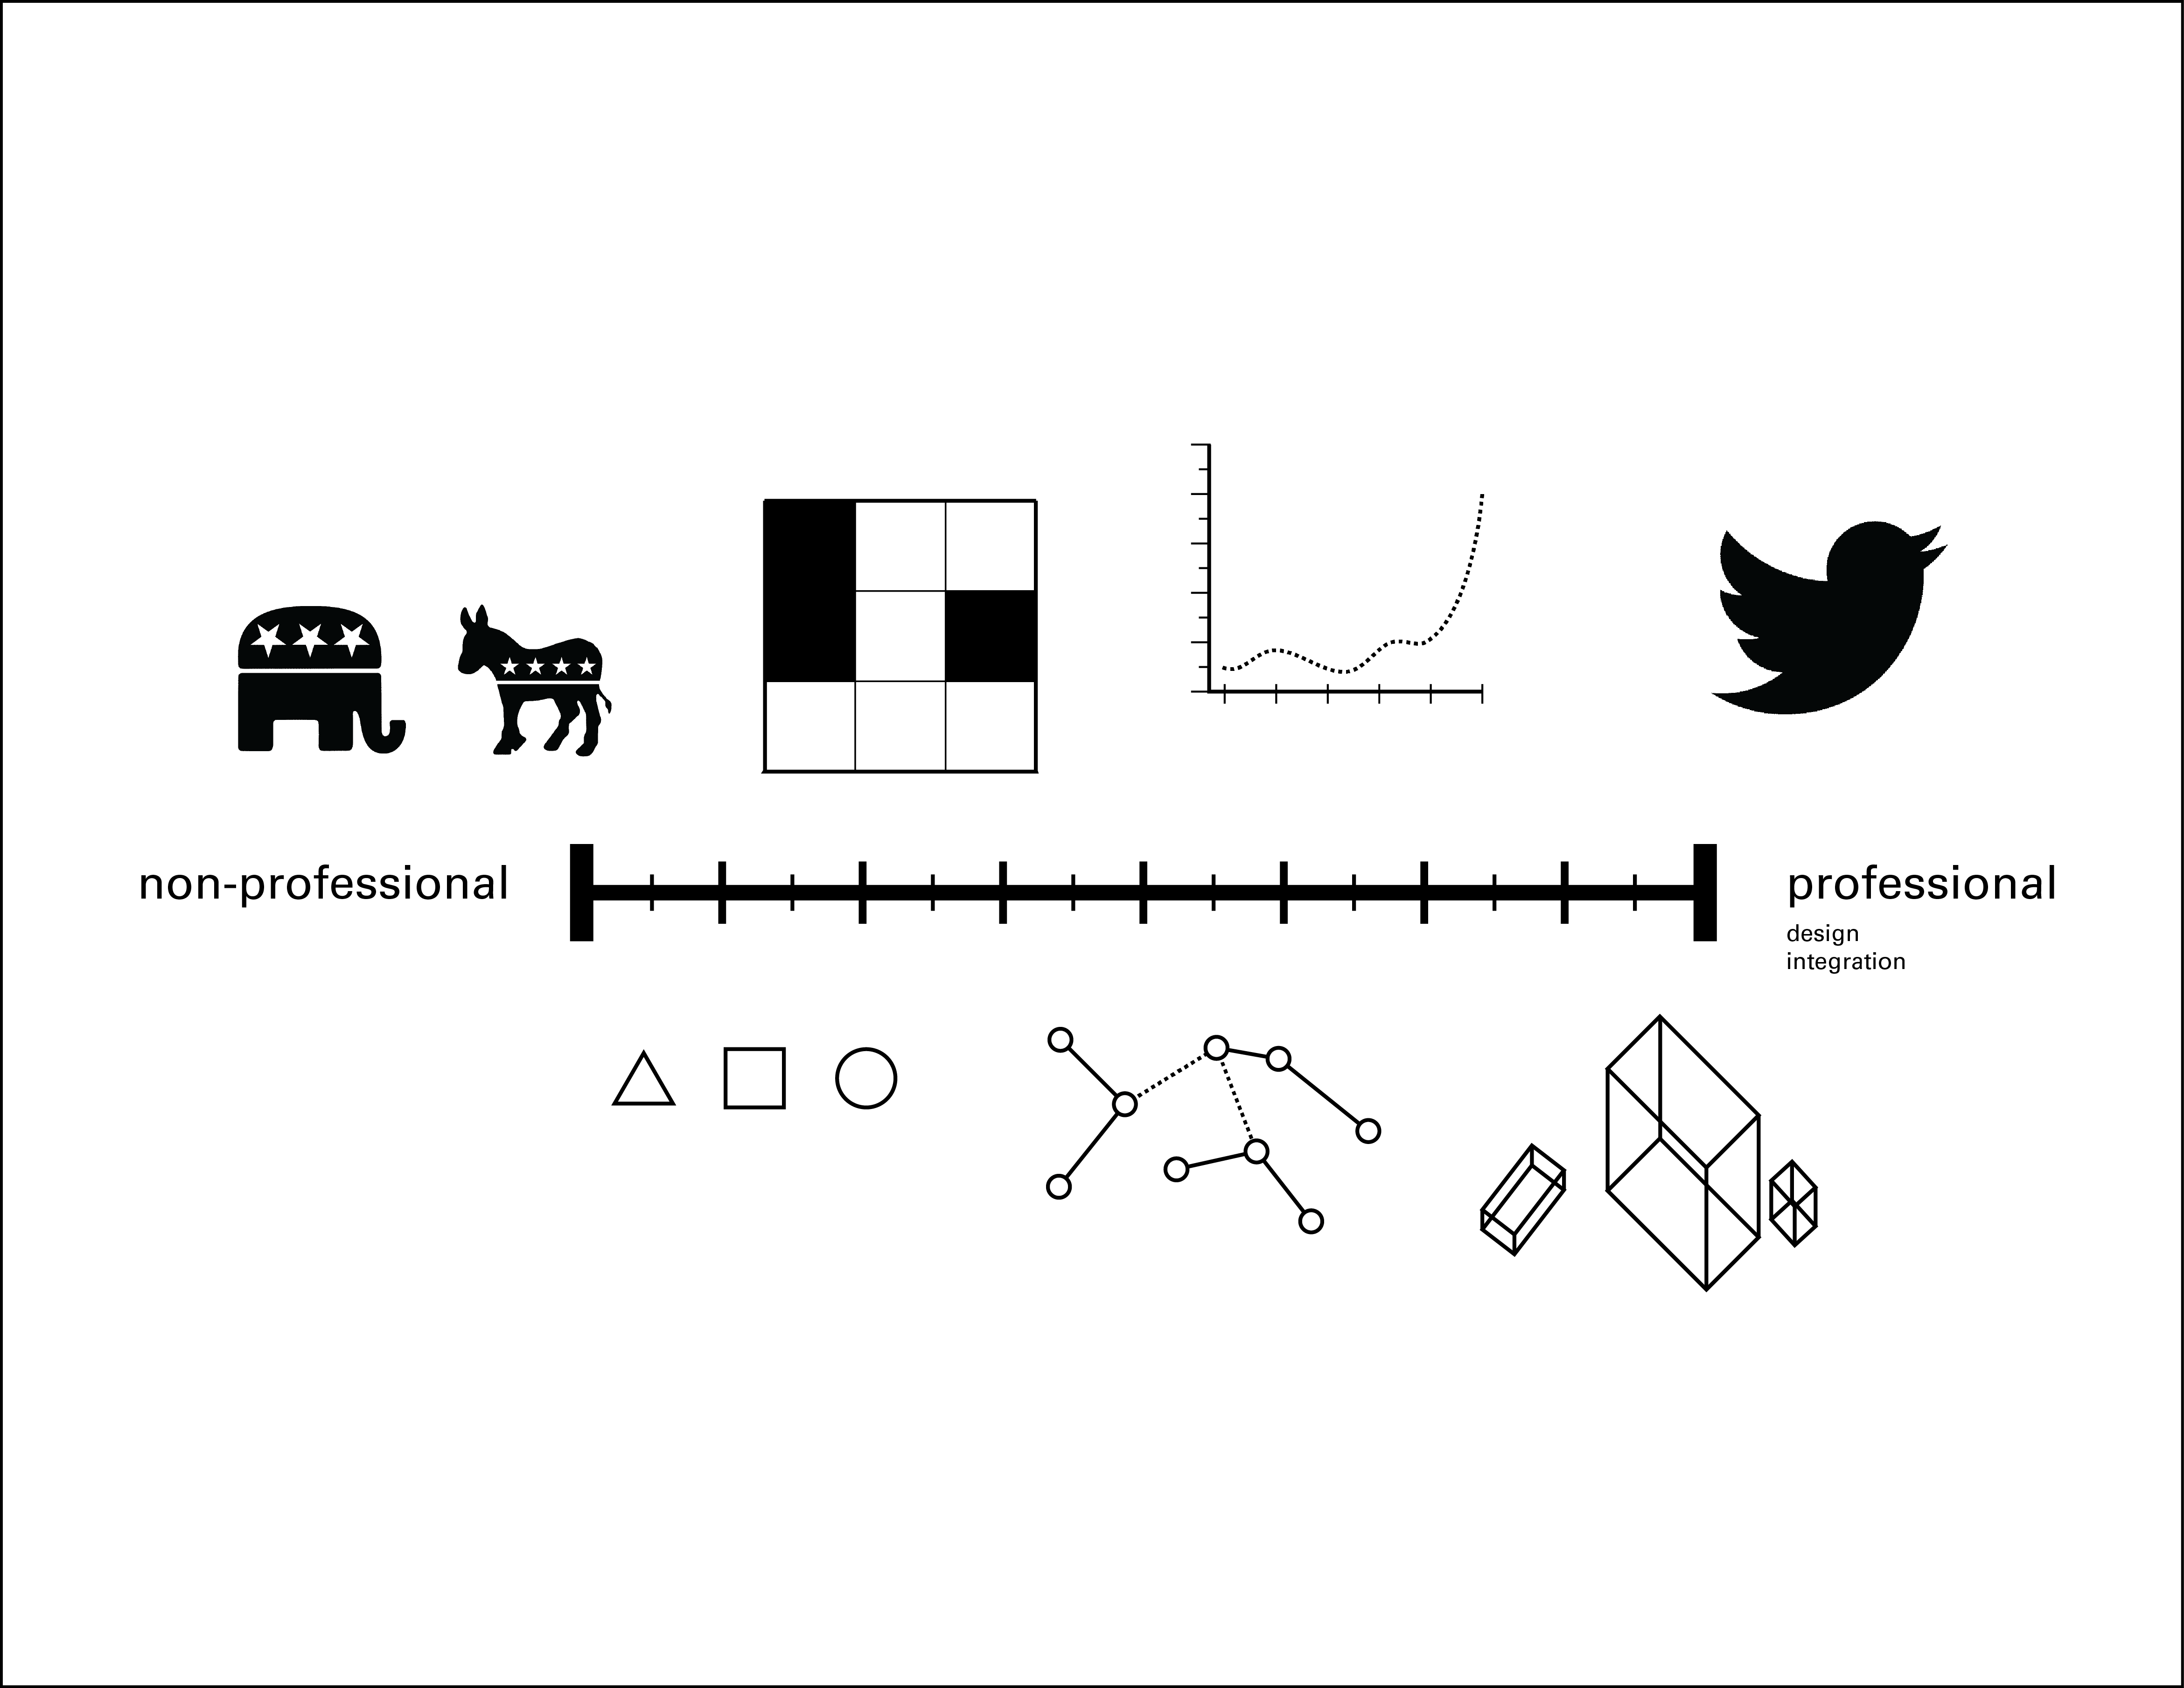
\includegraphics[width=\textwidth]{chapters/2/fig/spectrum.png}               
  \caption[number of bits per transaction]{
  The smaller the amount (bits) of information processed within one transaction,
  the easier to process. As it gets larger, it becomes unstructured data, which is hard to directly convert to a decision or
  intervention. Numbers indicate the average amount of information for each method of interaction.
  Note that that there is `unconstrained' methods, which the information is unlimited.
  }
  \label{fig:spectrum}
\end{figure}
The other side of the spectrum has the richest information and can be seen in organized events to gather people in one place which includes workshops, focus groups, \dots etc. Although these events are organized and centralized to make it effective for the head of the pyramid to listen, events are open ended, vocal, and unstructured, making it difficult to know the influence on the proposals the city made. \hlcyan{We can seek a form of interaction that is more communicative than a vote, but more structured than open discussion.} In any case, this information can be exchanged between participants, and it is influenced by what kind of media is used for this method.
\begin{figure}[!htb]
    
\includegraphics[width=\textwidth]{chapters/2/fig/unstructured_app.png}               
    \caption[diagram: unstructured app]{
        Modern technology enables the community to provide data in a centralized way through
        collaborative data collection and analysis.
        Compared to the methods that do not leverage the media technology,
        these are better at collecting more data at once,
        since there are no physical constraints for gathering.
        }
  \label{fig:unstructured_app}
\end{figure}


\begin{marginfigure}[{0cm}]
  
\includegraphics[width=\textwidth]{chapters/1/fig/hearings.png}               
  \repeatcaption{fig:hearings}{Urban planners started different methods of ``hearings'' to centralize input from the community. Appendix \ref{app:traditional} shows different traditional methods}
\end{marginfigure}

Different types of media technology influence these methods of hearing. Talking to each other is the least constrained, which again is unstructured, but rich.

\section{Professionals and citizens}

\begin{figure}[!htb]
  
\includegraphics[width=\textwidth]{chapters/2/fig/internalized_plan.png}               
  \caption[diagram: unstructured app]{Despite the innovation in ``hearing'' methods, this state still has the plan internalized in the top section of the pyramid.}
  \label{fig:internalized_plan}
\end{figure}

Until this point, the ``plan'' or the process of planning is still internalized inside the top sector. (Figure \ref{fig:internalized_plan}) \hlcyan{Both the planner side and the community demanded to externalize this element and make it visible to everyone}.

\subsection{the planning side and the ``wicked problem''}\label{subsec:wicked}

The difficulty and complexity of social planning was addressed by Churchman which coined the term ``wicked problems'' \cite{churchman1967guest}. Churchman first points there are `tame problems', which the issues are well defined and it is clear whether the problem was solved. `Wicked problems' are the opposite, which cannot be framed in a template and are difficult to validate whether the problem was solved.  \hlcyan{We can see the frustration that planners experience in Churchman's description:}
\begin{quotation}
The lay customers are complaining because planners and other professionals have not succeeded in solving the problems they claimed they could solve.
\end{quotation}
According to Churchman, there are ten characteristics of a `wicked problem', and one of them `The social planner has no right to be wrong' challenges the position of the planner.

Similar to the contrast of `tame' and `wicked' problems, other fields of science also questioned the performance difference of professionals solving problems compared to people that are nonprofessionals. Johnson states this by the cognitive science and artificial intelligence showing results that experts perform better compared to novices while the empirical research in behavioral decision claims that \hlcyan{this is not always true}. \cite{chi2014nature} He continues that artificial intelligence focuses on structured `tame' problems like chess, where the behavioral science looks into `wicked' issues that are hard to define the aspects and detangle the influences of each of them, such as predicting the market. Hence, this has created a discrepancy of the evaluation of the performance of experts. 
\hlcyan{Johnson cites Armstrong that suggests to hire the cheapest expert, pointing their poor performance in forecasting.}\cite{armstrong1978longrange} \hlcyan{Urban planning is one of social planning, which by nature is a ``wicked problem'', which means the urban planning experts could not be guaranteed to always preform better than novices.} 

% TODO: change 'hearings' to 'community meetings'
\begin{figure}[htb]
  
\includegraphics[width=\textwidth]{chapters/2/fig/externalized_plan.png}               
  \caption[diagram: externalized plan]{The plan has been externalized to the public. We see this by the current planning schema required to have a public meeting. (Although the strength of influence varies place to place.)}
  \label{fig:externalized_plan}
\end{figure}

\hlcyan{When planners are not able to meet public demands and are unable to predict what comes next, the gap of mistrust between public and experts increases.} \hlcyan{Especially when the value judgment is based on }Churchman's point in 1957 ``solutions to wicked problems are not true or false, but good or bad.''

One possible method to overcome "wicked problems" is to take
a collaborative approach. \cite{roberts2000wicked}
\footnote{The study examines three approaches, and concludes that the collaborative strategy is most effective.
  \begin{itemize}
\item Authoritative Strategies
\item Competitive Strategies
\item Collaborative Strategies
  \end{itemize}
}

Yet skills of collaboration are limited, especially among people who work in a traditional bureaucracy with a strong hierarchy limiting participation and team-based approaches to problem solving and decision making.

To overcome this, new tools and methods are needed to support collaboration, inform people with different perspectives, lower the administrative transaction cost, and provide a learning experience on each topic, which is exactly an effective democratic process. (Figure\ref{fig:externalized_plan})

\subsection{Democratization}

There is evidence that urbanization triggers democratic change\cite{woolley2010evidence} and as \hlcyan{urbanization is seen globally, we can assume that demands for democratization will generally increase.} Dewey advocated giving the community the power and right to collectively govern themselves, inferred that information and education are the key factors to have the community undergo decision making, and added that the `new journalist' was the one to coordinate. \cite{dewey2012public} 

He emphasizes that the `new journalist' has two central roles: verify which information is reliable; order it so the people can grasp
it efficiently.\footnote{In a modern world, a system may be able to do both using collective input.}
Shirky has pointed out that, historically, the balance between media consumption and creation from the community was dominated towards consumption, but the advent of modern communication tools and the amount of output processed from them show people also have the desire to create and share\cite{shirky2008here}. \hlcyan{We might see ``new journalism'' as a device that moderates between creation and consumption, forming a new type of system.} The challenge is to transform individual experiences, frameworks, and perspectives into a shared, understandable, and, most importantly, a transmittable area of knowledge


\begin{figure}[htb]
  
\includegraphics[width=\textwidth]{chapters/2/fig/community_engagment.png}               
  \caption[diagram: community engagement]{Community engagement that will directly influence the plan.}
  \label{fig:communityengagement}
\end{figure}

Figure \ref{fig:communityengagement} shows that people are now not only exposed the plan, but are able to provide feedback. As of 2017, it is required by Cambridge law to open a public meeting in order to obtain a permit. Again, the level of participation has been increasing and present planning procedure name this activity as the community engagement process.

\subsection{Analysis and Synthesis}
Yet the community has \hlcyan{one more step to become politically autonomous: the synthesis phase.}\hlcyan{In Athenian direct democracy, people not only voted, but proposed the topics to vote on.} In \underline{Notes on the Synthesis of Form}, Christopher Alexander clearly distinguishes that in a design procedure, there is always the analysis phase before the synthesis phase, and the two are different.


\begin{quotation}
Finding the right design program for a given problem is the first phase of the design process. It is, if we like, the analytic phase of the process. The first phase of the process must of course be followed by the synthetic phase, in which a form is derived from the program. We shall call this synthetic phase the realization of the program. \cite{alexander1964notes}
\end{quotation}

There are few attempts that distinguish these two processes. Having the premise that these two are different, there are fewer attempts to integrate them into the same platform. Figure\ref{fig:collective_design} shows one example of such a platform.
\hlcyan{The synthetic phase referred by architects was often a process done by an individual, which is a process of deciding trade offs and find the right configurations that most fits the context of a given problem. By inventing {\underline{the Pattern Language}}, Alexander created a method to synthesize an architecture plan through a deliberation process.{\cite{schulerpattern}}}

\begin{figure}[htb]
  
\includegraphics[width=\textwidth]{chapters/2/fig/bikebump.png}               
  \caption[diagram: integrated collective design]{Integrated design method that combines analytic and synthetic phases.}
\label{fig:collective_design}
\end{figure}


\subsection{Extending Collective Intelligence}
Artificial intelligence has been gaining attention because these technologies have advanced through the increase of available data as training sets. A substantial amount of data for training machines originates from human input, which is at the same time used for training (learn and teach) humans. Today we know this is a form of collective intelligence, which the inputs from the citizens are included in this category. Extended intelligence is a concept to acknowledge that intelligence was always a network and should incorporate both artificial intelligence and collective intelligence to utilized them mutually.\cite{pubpub:extended} Hidalgo points out that network intelligence existed from the beginning and cities are ``pockets where our species accumulates the capacity to produce information''.\cite{hidalgo2015information} He mentions that the novelty is today's technological context where computational resources have been distributed more than ever before.\cite{pubpub:whatsnew} Research says that the combination of these two types of intelligence has potential to overcome the performance\cite{baharad2011distilling} in fields that were thought to have little or no difference comparing professionals and nonprofessionals. (p\pageref{subsec:wicked}) With the collective and the artificial intelligence combined, the tool will now \hlcyan{learn} and augment the community.